\documentclass[conference]{IEEEtran}
\usepackage{fontspec}
\setmainfont{TeX Gyre Termes}
\usepackage{amsmath,amssymb}
\usepackage{graphicx}
\usepackage{booktabs}
\usepackage{url}
\usepackage[hidelinks]{hyperref}
\newcommand{\dd}{\mathrm{d}}
\renewcommand{\IEEEkeywordsname}{Từ khóa}
\renewcommand{\abstractname}{Tóm tắt}
\renewcommand{\tablename}{BẢNG}
\renewcommand{\figurename}{Hình}
\renewcommand{\refname}{Tài liệu tham khảo}
\begin{document}

\title{Giá trị gia tăng của MRI lặp trong dự báo sa sút trí tuệ ở người suy giảm nhận thức nhẹ: mô hình landmark kiểm duyệt khoảng trên ADNI}

\author{\IEEEauthorblockN{Nhóm nghiên cứu Ngày hội Kỹ thuật}
\IEEEauthorblockA{Cơ sở lý thuyết phiên bản 2 · Kiểm chứng nội bộ · 25/11/2026}}

\maketitle

\begin{abstract}
Ở người suy giảm nhận thức nhẹ (MCI) chưa điều trị đặc hiệu, liệu chụp lại MRI để đo tốc độ teo hồi hải mã có cải thiện dự báo sa sút trí tuệ so với chỉ theo dõi nhận thức – chức năng? Chúng tôi xây dựng mô hình landmark nhiều mốc, xem kết cục là kiểm duyệt khoảng vì Dementia chỉ được ghi nhận tại lượt tái khám, đo tốc độ teo bằng slope co rút (BLUP) và đánh giá bốn mô hình lồng nhau M0–M3 trên cùng tập mốc. Dữ liệu ADNI được chia 80/20 theo người. Kiểm định chéo lặp 5 fold × 20 lần trên 555 người (1.169 mốc) cho td-AUC ở 730 ngày từ 0,871 (M0) đến 0,886 (M3). Chênh lệch M3 − M2 là 0,004 (KTC 95\% −0,008 đến 0,014) và chênh lệch net benefit ở ngưỡng 15–30\% là 0,001 (−0,010 đến 0,010); theo quy tắc định trước, kết luận là bất định ở 730 ngày và tương đương ở 1.095 ngày. Tốc độ hai điểm kiểu phiên bản trước không thêm thông tin (ΔAUC −0,003). Bỏ qua kiểm duyệt khoảng làm Cox dự báo thấp gần một nửa nguy cơ ở 365 ngày (O/E 1,84). Trên tập test 141 người, kết quả nhất quán nhưng kém chính xác.
\end{abstract}

\begin{IEEEkeywords}
ADNI, MCI, MRI cấu trúc, landmarking, kiểm duyệt khoảng, BLUP, net benefit, TRIPOD+AI.
\end{IEEEkeywords}

\section{Giới thiệu}
Năm 2024, Alzheimer's Association công bố tiêu chí chẩn đoán và phân giai đoạn dựa trên sinh học, bổ sung biểu hiện máu~\cite{jack2024}. Tháng 5/2025, FDA cấp phép xét nghiệm máu pTau217/Aβ1-42 đầu tiên~\cite{fda2025}. Người dùng kháng thể kháng amyloid được chụp MRI nhiều lần để theo dõi ARIA~\cite{ema}, nhưng điều trị này gây mất thể tích não ngoài dự kiến (ARPA)~\cite{belder2024}. Vì vậy câu hỏi thực tế không còn là MRI có dự báo được hay không, mà là: ở người MCI \emph{chưa} điều trị, một lần MRI lặp có thêm giá trị tiên lượng so với theo dõi nhận thức hay không.

Phiên bản trước (v1) dùng Cox kiểm duyệt phải, một mốc mỗi người, tốc độ teo từ hai lần chụp cách nhau ≥ 90 ngày và tập test 120 người với 10 ca ở 365 ngày. Bản này sửa ba điểm yếu đã kiểm chứng trên dữ liệu: (i) nhãn bị kiểm duyệt khoảng; (ii) tốc độ hai điểm bị nhiễu đo chi phối; (iii) cỡ mẫu đánh giá quá nhỏ. Đóng góp gồm: một khung landmark kiểm duyệt khoảng có trọng số theo người; slope BLUP thay cho hiệu hai điểm; và quy tắc kết luận ba nhánh theo ngưỡng δ định trước, báo cáo theo TRIPOD+AI~\cite{tripod}.

\section{Dữ liệu và đoàn hệ}
\subsection{Nguồn và phân hoạch}
Bộ dữ liệu gồm 20 bảng CSV của ADNI~\cite{adni} (ADNI1, GO, 2, 3 và 4: DXSUM, PTDEMOG, MMSE, FAQ, ADAS, NEUROBAT, UCSFFSX7 (FreeSurfer 7.2/7.4.1), FOXLABBSI và các bảng phụ). Phân hoạch theo RID được đóng băng từ v1. Train có 4.073 RID (80\%), test có 1.020 RID (20\%), không có RID chung. Mọi bước học, chọn siêu tham số và kiểm định chéo chỉ dùng train.

\subsection{Mốc landmark và kết cục kiểm duyệt khoảng}
Theo nguyên lý landmarking~\cite{landmark}, mỗi lượt chẩn đoán MCI ngoài screening, chưa từng có Dementia và còn ít nhất một lượt sau đó, là một mốc $s$. Đại lượng dự báo là
\begin{equation}
\pi_i(s,h)=P\big(T_i\le s+h \mid T_i>s,\,Z_i(s)\big),
\end{equation}
với $h\in\{365,730,1095\}$ ngày và $Z_i(s)$ chỉ dùng dữ liệu có ngày $\le s$. Dementia chỉ được biết là xảy ra trong $(L_i,R_i]$: $L$ là lượt cuối chưa Dementia, $R$ là lượt Dementia đầu tiên ($R=\infty$ nếu chưa ghi nhận). Theo dõi bị cắt hành chính ở 1.095 ngày.

Hình~\ref{fig:heap} cho thấy ngày ghi nhận dồn thành cụm theo lịch tái khám. Trên bộ dữ liệu đầy đủ, độ rộng khoảng $(L,R]$ có trung vị 360 ngày. Ở $h=365$, số ca có khoảng vắt qua chân trời (111) nhiều hơn số ca ghi nhận trước đó (89). Tỷ lệ ca bất định giảm từ 56\% ở 365 ngày xuống 27\% ở 730 ngày. Vì lý do cấu trúc này, độc lập với kết quả mô hình, chân trời chính được chọn là 730 ngày.

\begin{figure}[t]
\centering
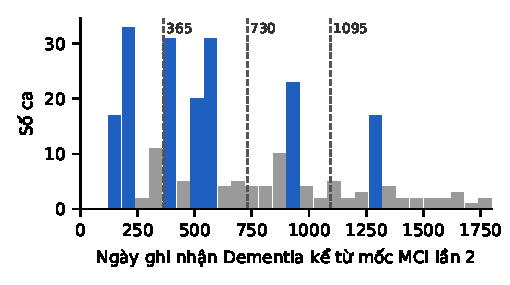
\includegraphics[width=\columnwidth]{fig1_heaping.pdf}
\caption{Ngày ghi nhận Dementia sau mốc MCI lần 2 trong train (206 ca trong 1.095 ngày). Các cụm trùng lịch khám 6–12 tháng.}
\label{fig:heap}
\end{figure}

\section{Đặc trưng}
\subsection{Vì sao tốc độ hai điểm thất bại}
Nếu mỗi lần phân đoạn có sai số độc lập phương sai $\sigma^2$, tốc độ năm hóa từ hai lần chụp có phương sai sai số
\begin{equation}
\operatorname{Var}(\hat r-r)=2\sigma^2\Big(\tfrac{365{,}25}{d_2-d_1}\Big)^2 .
\end{equation}
Trong Cox, sai số cộng tính kéo hệ số về 0 theo tỷ số $\operatorname{Var}(r)/[\operatorname{Var}(r)+\operatorname{Var}(\hat r-r)]$. Trong train, khoảng cách hai lần chụp có trung vị 208 ngày. Độ lệch chuẩn tốc độ hai điểm là 426 mm³/năm, trong khi trung bình teo của quần thể MCI chỉ 110 mm³/năm.

\subsection{Đặc trưng v2}
Thể tích hồi hải mã (ST29SV+ST88SV) được hiệu chỉnh ICV bằng phương pháp phần dư, với $b$ ước lượng trên 846 người luôn CN trong train:
$\mathrm{HV_{adj}}=\mathrm{HV}-b(\mathrm{ICV}-\overline{\mathrm{ICV}}_{\mathrm{CN}})$.
Slope được tính bằng BLUP từ mô hình hỗn hợp $y_{ij}=(\gamma_0+u_{0i})+(\gamma_1+u_{1i})t_{ij}+\varepsilon_{ij}$, dùng mọi lần đo trước hoặc tại mốc, trải ≥ 300 ngày. Với MRI, chỉ dùng các lần chụp cùng phiên bản FreeSurfer và cùng cường độ từ trường:
\begin{equation}
\hat r_i=\gamma_1+\big[D X_i^\top V_i^{-1}(y_i-X_i\gamma)\big]_2,\quad V_i=X_i D X_i^\top+\sigma^2 I .
\end{equation}
Các tham số $\gamma$, $D$ và $\sigma^2$ được ước lượng bằng moment trên người MCI của train rồi khóa lại. Bước này không dùng kết cục. Độ lệch chuẩn của slope BLUP hồi hải mã là 63 mm³/năm, so với 426 mm³/năm của tốc độ hai điểm.

Bốn tập biến lồng nhau gồm:
\begin{itemize}
\item \textbf{M0:} $\tau(s)$ (năm từ MCI đầu tiên), $\tau^2$, tuổi, giới, học vấn, MMSE, FAQ, ADAS-Cog13, RAVLT trì hoãn 30 phút (trong 45 ngày trước mốc).
\item \textbf{M1:} M0 cộng $\mathrm{HV_{adj}}$, độ dày nội khứu và chỉ báo 3T (MRI trong 365 ngày trước mốc).
\item \textbf{M2:} M1 cộng slope ADAS-Cog13 và slope FAQ.
\item \textbf{M3:} M2 cộng slope hồi hải mã và slope nội khứu.
\end{itemize}

\section{Mô hình}
Mô hình tỷ lệ nguy cơ có nguy cơ nền hằng từng khúc trên sáu khúc 182,5 ngày:
$S(t\mid z)=\exp[-H_0(t)e^{\beta^\top z}]$, $H_0(t)=\sum_k e^{a_k}\,|[0,t]\cap I_k|$.
Mỗi mốc đóng góp xác suất rơi vào đúng khoảng quan sát:
\begin{equation}
\begin{aligned}
\ell={}&\textstyle\sum_k w_k\log\big[S(L_k\mid z_k)-S(R_k\mid z_k)\big]\\
&-\tfrac{\lambda}{2}\lVert\beta\rVert^2-\tfrac{\kappa}{2}\textstyle\sum_j(a_j-a_{j-1})^2 ,
\end{aligned}
\end{equation}
với trọng số $w_k=1/n_i$ để mỗi người có tổng trọng số 1 dù đóng góp $n_i$ mốc. Nếu không có trọng số này, người ổn định nhiều mốc chi phối và nguy cơ nền bị kéo xuống. $\lambda\in\{0{,}1;1;10\}$ được chọn bằng CV lồng 3 fold theo log-likelihood khoảng ngoài fold. Gradient được tính giải tích và kiểm tra bằng sai phân hữu hạn (sai số tương đối $3\times10^{-9}$). Kiểm duyệt được mô hình hóa bằng Cox ridge~\cite{cox} có trọng số theo người, với các hiệp biến $\tau$, tuổi, MMSE, ADAS-Cog13 và FAQ.

\section{Đánh giá}
Tại chân trời $h$, mỗi mốc được xếp vào một trong ba nhóm:
\begin{itemize}
\item \textbf{Ca:} $R\le h$.
\item \textbf{Đối chứng:} $L\ge h$.
\item \textbf{Bất định:} $L<h<R$. Thời điểm $T$ được rút trong $(L,R]$ từ mô hình tham chiếu M0, chung cho mọi mô hình nên không thiên vị M3.
\end{itemize}
Trọng số IPCW là $1/\hat G(R^-)$ cho ca và $1/\hat G(h)$ cho đối chứng. Các chỉ số gồm td-AUC có trọng số, Brier và IPA $=1-\mathrm{Brier}/\mathrm{Brier}_{\text{null}}$~\cite{ipa}, và net benefit~\cite{dca}:
\begin{equation}
\mathrm{NB}(p_t)=\tfrac{\mathrm{TP}}{n}-\tfrac{\mathrm{FP}}{n}\cdot\tfrac{p_t}{1-p_t}.
\end{equation}
NB$_{\text{core}}$ là trung bình NB ở các ngưỡng 15, 20, 25 và 30\%.

Trên dữ liệu thật, tỷ lệ quan sát theo IPCW ở 730 ngày (0,34) cao hơn ước lượng Kaplan–Meier (0,28). Mô phỏng từ mô hình đã khớp với kiểm duyệt độc lập cho slope hiệu chuẩn 0,99, cho thấy cơ chế đúng khi giả định IPCW thỏa mãn. Vì vậy hiệu chuẩn được đánh giá không phụ thuộc mô hình: O/E và slope trên 5 nhóm nguy cơ, với giá trị quan sát là Kaplan–Meier có biến cố tại điểm giữa khoảng. Các chênh lệch Δ giữa mô hình dùng chung $y$ và $w$ nên vẫn so sánh công bằng.

\textit{Thiết kế:} Kiểm định chéo lặp 5 fold × 20 lần chia theo RID. Mỗi fold đánh giá một mốc ngẫu nhiên mỗi người. Δ là trung bình qua các lần lặp; KTC 95\% lấy từ 1.000 lần bootstrap theo cụm người, mỗi vòng rút một lần lặp.

\textit{Quy tắc kết luận định trước} cho Δ = M3 − M2:
\begin{itemize}
\item \textbf{Có giá trị gia tăng:} cận dưới ΔAUC $>0$, ΔAUC $\ge 0{,}02$ và cận dưới ΔNB$_{\text{core}}>0$.
\item \textbf{Tương đương:} KTC của ΔAUC nằm trong $(-0{,}02;\,0{,}02)$ và cận trên ΔNB$_{\text{core}}\le 0{,}01$.
\item \textbf{Bất định:} các trường hợp còn lại.
\end{itemize}
Tập test được chấm một lần bằng mô hình khóa, với 20 lần rút mốc và đa bội.

\section{Kết quả}
\subsection{Đoàn hệ}
Trong train có 3.644 mốc từ 1.015 người. Tập phân tích ghép cặp đủ biến M3 gồm 1.169 mốc từ 555 người, trong đó 171 người có Dementia trong cửa sổ. Độ bao phủ thu hẹp dần qua các mô hình: M0 có 863 người, M1 có 809, M2 có 602 và M3 có 555. Ràng buộc chính là yêu cầu chuỗi đo trải ≥ 300 ngày. Tập test có 141 người đủ M3, tương ứng 305 mốc.

\subsection{Hiệu năng trong kiểm định chéo}
Bảng~\ref{tab:cv} cho thấy cả bốn mô hình phân biệt tốt (AUC 0,86–0,90) và hiệu chuẩn tổng thể sát (O/E 0,94–1,00). Slope hiệu chuẩn Kaplan–Meier là 1,2–1,4: mô hình hơi dè dặt ở hai đầu nguy cơ. Ở 730 ngày, mọi mô hình có NB$_{20\%}$ (0,245–0,255) cao hơn chiến lược can thiệp tất cả (0,172).

\begin{table}[t]
\caption{Kiểm định chéo lặp trên train (555 người, trung bình 20 lần lặp)}
\label{tab:cv}
\centering\footnotesize
\begin{tabular}{@{}llccccc@{}}
\toprule
$h$ & Mô hình & AUC & IPA & O/E & Slope & NB$_{\text{core}}$\\
\midrule
365 & M0 & 0,864 & 0,279 & 1,00 & 1,41 & 0,133\\
    & M3 & 0,870 & 0,294 & 1,00 & 1,32 & 0,138\\
730 & M0 & 0,871 & 0,361 & 0,98 & 1,29 & 0,235\\
    & M1 & 0,881 & 0,388 & 0,97 & 1,22 & 0,244\\
    & M2 & 0,882 & 0,392 & 0,98 & 1,24 & 0,244\\
    & M3 & 0,886 & 0,402 & 0,97 & 1,22 & 0,245\\
1095& M0 & 0,885 & 0,413 & 0,95 & 1,24 & 0,264\\
    & M3 & 0,902 & 0,462 & 0,94 & 1,18 & 0,274\\
\bottomrule
\end{tabular}
\end{table}

\subsection{Giá trị gia tăng}
Bảng~\ref{tab:delta} trình bày các chênh lệch ghép cặp. MRI hiện tại (M1 − M0) đóng góp nhiều nhất: +0,011 AUC ở 730 ngày, với khoảng tin cậy vẫn chứa 0. Slope nhận thức (M2 − M1) gần như không thêm gì. Với slope MRI (M3 − M2) ở 730 ngày, ΔAUC là 0,004 (−0,008 đến 0,014) và ΔNB$_{\text{core}}$ là 0,001 (−0,010 đến 0,010). Cận trên ΔNB vượt 0,01 rất ít, nên kết luận định trước là \emph{bất định}. Ở 1.095 ngày, kết luận là \emph{tương đương}.

\begin{table}[t]
\caption{Chênh lệch ghép cặp ở 730 ngày (KTC 95\% bootstrap cụm)}
\label{tab:delta}
\centering\footnotesize
\begin{tabular}{@{}lcc@{}}
\toprule
So sánh & ΔAUC & ΔNB$_{\text{core}}$\\
\midrule
M1 − M0 & 0,011 (−0,007; 0,029) & 0,009 (−0,005; 0,021)\\
M2 − M1 & 0,001 (−0,007; 0,008) & 0,001 (−0,006; 0,008)\\
M3 − M2 & 0,004 (−0,008; 0,014) & 0,001 (−0,010; 0,010)\\
M3 − M2, 1.095 ngày & 0,005 (−0,010; 0,017) & 0,000 (−0,010; 0,009)\\
Test: M3 − M2 & −0,002 (−0,020; 0,015) & −0,006 (−0,022; 0,011)\\
\bottomrule
\end{tabular}
\end{table}

\subsection{Phân tích độ nhạy}
Hình~\ref{fig:forest} tóm tắt các phân tích độ nhạy:
\begin{itemize}
\item \textbf{S1 (Cox kiểm duyệt phải):} AUC giữ nguyên, nhưng ở 365 ngày nguy cơ bị dự báo thấp gần một nửa (O/E 1,84 so với 1,02), IPA giảm từ 0,272 xuống 0,142 và ΔNB$_{\text{core}}$ là −0,048 (−0,070; −0,027).
\item \textbf{S2a:} tốc độ hai điểm kiểu v1 không thêm thông tin (ΔAUC −0,003).
\item \textbf{S2b:} ở phân nhóm ADNIGO/2 (235 người, chụp 3T đồng nhất), slope BLUP cho ΔAUC 0,038 (0,010; 0,072) và ΔNB 0,024 (0,006; 0,041). BSI hồi hải mã~\cite{bsi} thì không thêm thông tin (0,005).
\item \textbf{S3, S4, S5} (mốc MCI lần 2; Dementia xác nhận; bỏ FAQ) đều cho Δ dương nhỏ, với khoảng tin cậy chứa 0.
\end{itemize}

\begin{figure}[t]
\centering
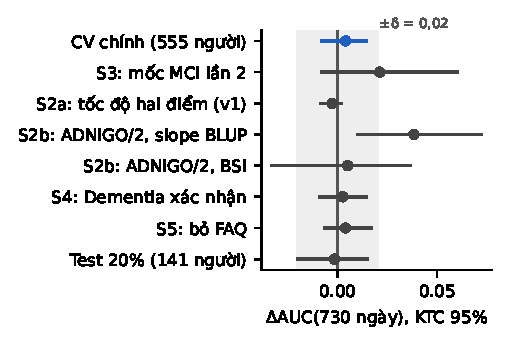
\includegraphics[width=\columnwidth]{fig2_forest.pdf}
\caption{ΔAUC (M3 − M2, hoặc biến thay thế − M2) ở 730 ngày. Vùng xám là ±δ.}
\label{fig:forest}
\end{figure}

\subsection{Tập test 20\%}
Trên 141 người, AUC ở 730 ngày là 0,917–0,924 và O/E là 1,03–1,06. Hiệu chuẩn theo nhóm bám đường chéo, chỉ hơi thấp ở nhóm nguy cơ cao (Hình~\ref{fig:cal}). Chênh lệch M3 − M2 là −0,002 (−0,020; 0,015), kết luận bất định do cỡ mẫu. Phân nhóm mốc MCI lần 2 trên test chỉ có 23 người nên không được báo cáo.

\begin{figure}[t]
\centering
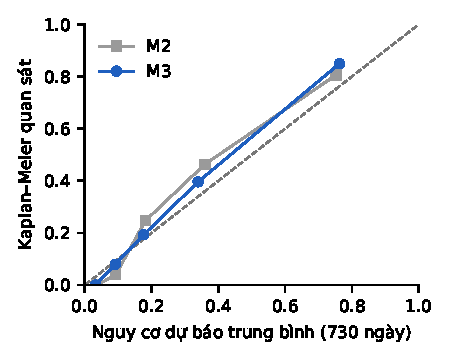
\includegraphics[width=0.85\columnwidth]{fig3_calibration.pdf}
\caption{Hiệu chuẩn trên test ở 730 ngày: 5 nhóm nguy cơ, quan sát bằng Kaplan–Meier.}
\label{fig:cal}
\end{figure}

\section{Thảo luận}
Khi nhiễu đo được kiểm soát bằng BLUP và kết cục được mô hình hóa đúng, MRI lặp không thêm giá trị tiên lượng đủ lớn trên toàn đoàn hệ. Ước lượng điểm nằm xa dưới ngưỡng δ = 0,02, và ở 1.095 ngày kết luận tương đương. Đóng góp chính đến từ một lần MRI hiện tại cùng nhận thức tại mốc. Phân nhóm ADNIGO/2 gợi ý slope có ích khi chuỗi ảnh đồng nhất về máy và giao thức. Đây là phân tích thăm dò với 5 lần lặp, cần kiểm chứng độc lập trước khi dùng để khuyến nghị.

S1 cho thấy giá trị thực tế của việc mô hình hóa kiểm duyệt khoảng. Mô hình khoảng không cải thiện xếp hạng, nhưng cải thiện xác suất tuyệt đối ở chân trời ngắn, mà chính xác suất này mới quyết định net benefit. Tốc độ hai điểm vô ích, phù hợp với phân tích pha loãng hồi quy ở mục III.

\textit{Giới hạn:}
\begin{itemize}
\item Nhãn Dementia của DXSUM không xác định căn nguyên.
\item Tử vong được xử lý như kiểm duyệt.
\item 97\% ảnh tại mốc chưa được QC thủ công.
\item IPCW lệch so với Kaplan–Meier trên dữ liệu thật, gợi ý kiểm duyệt phụ thuộc lịch khám.
\item Phân tích dùng ca đầy đủ; ADNI không đại diện cho người Việt Nam.
\item Phân hoạch test đã được xem ở v1; tập test nhỏ hơn cỡ mẫu khuyến nghị cho kiểm chứng~\cite{riley}.
\item Mô hình không áp dụng cho người đang dùng kháng thể kháng amyloid.
\end{itemize}

\section{Kết luận}
Với dữ liệu ADNI hiện có, chưa có bằng chứng rằng chỉ định MRI lặp chỉ để tiên lượng ở người MCI chưa điều trị đem lại lợi ích vượt ngưỡng lâm sàng. Kết luận ở 730 ngày là bất định, ở 1.095 ngày là tương đương. Một lần MRI cùng đánh giá nhận thức – chức năng đạt AUC khoảng 0,88 ở 2 năm. Bước tiếp theo là bổ sung amyloid/CDR/APOE và p-tau217 huyết tương, cùng kiểm chứng ngoài trên dữ liệu Việt Nam.

\begin{thebibliography}{10}\footnotesize
\bibitem{landmark} H. C. van Houwelingen, ``Dynamic prediction by landmarking in event history analysis,'' \emph{Scand. J. Stat.}, vol. 34, pp. 70--85, 2007.
\bibitem{cox} D. R. Cox, ``Regression models and life-tables,'' \emph{J. R. Stat. Soc. B}, vol. 34, no. 2, pp. 187--202, 1972.
\bibitem{jack2024} C. R. Jack Jr. et al., ``Revised criteria for diagnosis and staging of Alzheimer's disease: Alzheimer's Association Workgroup,'' \emph{Alzheimer's Dement.}, vol. 20, no. 8, pp. 5143--5169, 2024.
\bibitem{fda2025} U.S. FDA, ``FDA clears first blood test used in diagnosing Alzheimer's disease,'' 16 May 2025.
\bibitem{ema} European Medicines Agency, ``Leqembi (lecanemab): product information,'' 2025.
\bibitem{belder2024} C. R. S. Belder et al., ``Brain volume change following amyloid-beta immunotherapy for Alzheimer's disease: amyloid-removal-related pseudo-atrophy,'' \emph{Lancet Neurol.}, 2024.
\bibitem{tripod} G. S. Collins et al., ``TRIPOD+AI statement,'' \emph{BMJ}, vol. 385, e078378, 2024.
\bibitem{riley} R. D. Riley et al., ``Minimum sample size calculations for external validation of a clinical prediction model with a time-to-event outcome,'' \emph{Stat. Med.}, 2021.
\bibitem{bsi} P. A. Freeborough and N. C. Fox, ``The boundary shift integral,'' \emph{IEEE Trans. Med. Imaging}, vol. 16, no. 5, pp. 623--629, 1997.
\bibitem{dca} A. J. Vickers and E. B. Elkin, ``Decision curve analysis,'' \emph{Med. Decis. Making}, vol. 26, no. 6, pp. 565--574, 2006.
\bibitem{ipa} M. W. Kattan and T. A. Gerds, ``The index of prediction accuracy,'' \emph{Diagn. Progn. Res.}, vol. 2, 7, 2018.
\bibitem{adni} Alzheimer's Disease Neuroimaging Initiative, ``Diagnostic information,'' ADNI Documentation.
\end{thebibliography}

\end{document}
